\documentclass[french]{template}

% latex svg without inkscape
\usepackage[inkscapelatex=false]{svg}

\begin{document}

\titre{Projet de Théorie des Graphes}
\UE{Théorie des Graphes}
\enseignant{Riadh \textsc{Dhaou}}
\eleves{Leïlie \textsc{Canillac} \\ Vianney \textsc{Hervy}}

\fairemarges
\fairepagedegarde
\tabledematieres
\listedesfigures

\section*{Avant-propos}

Les figures \ref{fig:points} et \ref{fig:graph} montrent déjà la densité d'informations contenues dans ces graphes, leurs représentations graphiques risquent donc d'être peu lisibles. C'est pourquoi nous ne les avons pas toutes incluses dans ce rapport. Cepandant, elles sont toutes disponibles dans le dossier \texttt{doc/img} de ce projet.

\section{Partie 1 : Modélisation sous forme de graphe}

\begin{figure}[ht]
    \centering
    \begin{tabular}{|c|c|c|}
        \hline
        faible densité                                            &
        moyenne densité                                           &
        haute densité                                               \\
        \hline\hline
        
\includegraphics[width=0.3\textwidth]{img/low/points.png} &
        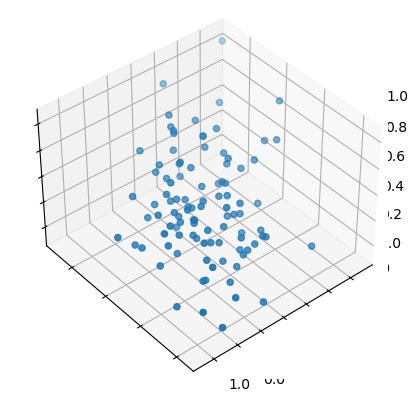
\includegraphics[width=0.3\textwidth]{img/avg/points.png} &
        
\includegraphics[width=0.3\textwidth]{img/high/points.png}  \\
        \hline
    \end{tabular}
    \caption{Représentations graphiques des essaims sans considération de portée}
    \label{fig:points}
\end{figure}

\begin{figure}[ht]
    \centering
    \begin{tabular}{|c|c|c|c|}
        \hline
        portée                                                         &
        faible densité                                                 &
        moyenne densité                                                &
        haute densité                                                    \\
        \hline\hline
        $20 000$ km                                                    &
        
\includegraphics[width=0.2\textwidth]{img/low/graph_20000.png} &
        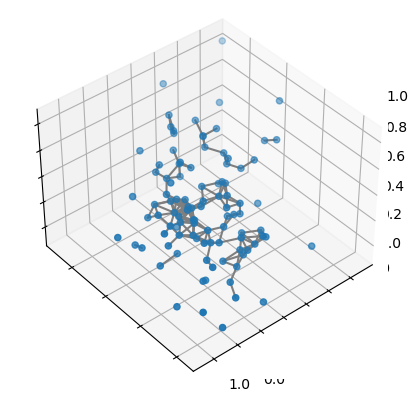
\includegraphics[width=0.2\textwidth]{img/avg/graph_20000.png} &
        
\includegraphics[width=0.2\textwidth]{img/high/graph_20000.png}  \\
        \hline
        $40 000$ km                                                    &
        
\includegraphics[width=0.2\textwidth]{img/low/graph_40000.png} &
        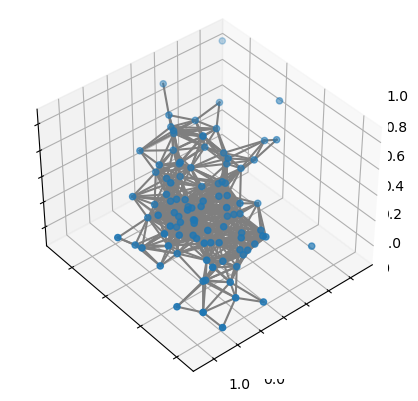
\includegraphics[width=0.2\textwidth]{img/avg/graph_40000.png} &
        
\includegraphics[width=0.2\textwidth]{img/high/graph_40000.png}  \\
        \hline
        $60 000$ km                                                    &
        
\includegraphics[width=0.2\textwidth]{img/low/graph_60000.png} &
        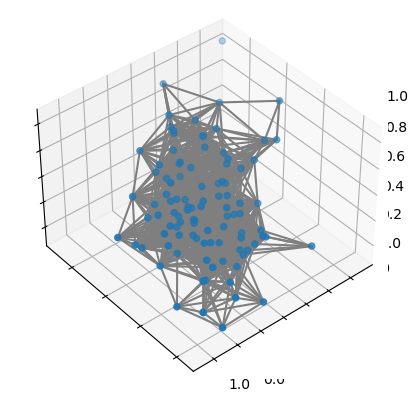
\includegraphics[width=0.2\textwidth]{img/avg/graph_60000.png} &
        
\includegraphics[width=0.2\textwidth]{img/high/graph_60000.png}  \\
        \hline
    \end{tabular}
    \caption{Représentations graphiques des graphes en fonction de la portée et de la densité}
    \label{fig:graph}
\end{figure}

\section{Partie 2 : Étude des graphes non-valués}

\subsection{Degrés}

\begin{figure}[ht]
    \centering
    \begin{tabular}{|c|c|c|c|}
        \hline
        portée      & faible densité & moyenne densité & haute densité \\
        \hline\hline
        $20 000$ km & $1.80$         & $3.46$          & $3.72$        \\
        \hline
        $40 000$ km & $11.42$        & $16.84$         & $18.68$       \\
        \hline
        $60 000$ km & $29.42$        & $35.64$         & $37.40$       \\
        \hline
    \end{tabular}
    \caption{Moyennes des degrés en fonction de la portée et de la densité}
    \label{tab:degrees-mean}
\end{figure}

Doutant sur la définition de "distribution du degré", nous avons à la fois représenté la distribution spatiale (figure \ref{fig:degrees}) et la distribution des valeurs (figure \ref{fig:degree-hist}).

La distribution spatiale du degré (figure \ref{fig:degrees}) n'a rien de surprenant. Plus la densité est forte et plus la portée est grande, plus les degrés sont élevés. On remarque aussi que les satellites situés près du centre du nuage ont tendance à avoir un degré plus élevé que ceux situés en périphérie.

\begin{figure}[ht]
    \centering
    \begin{tabular}{|c|c|c|c|}
        \hline
        portée                                                           &
        faible densité                                                   &
        moyenne densité                                                  &
        haute densité                                                      \\
        \hline\hline
        $20 000$ km                                                      &
        
\includegraphics[width=0.2\textwidth]{img/low/degrees_20000.png} &
        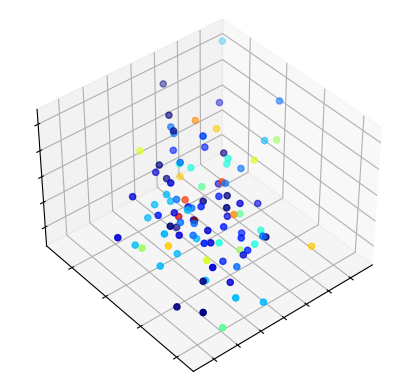
\includegraphics[width=0.2\textwidth]{img/avg/degrees_20000.png} &
        
\includegraphics[width=0.2\textwidth]{img/high/degrees_20000.png}  \\
        \hline
        $40 000$ km                                                      &
        
\includegraphics[width=0.2\textwidth]{img/low/degrees_40000.png} &
        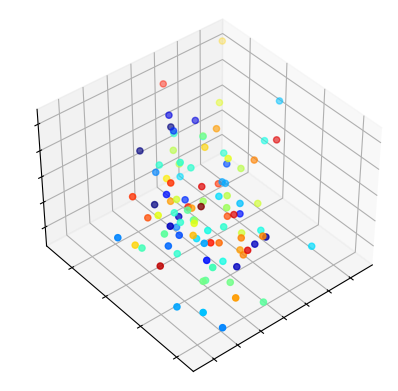
\includegraphics[width=0.2\textwidth]{img/avg/degrees_40000.png} &
        
\includegraphics[width=0.2\textwidth]{img/high/degrees_40000.png}  \\
        \hline
        $60 000$ km                                                      &
        
\includegraphics[width=0.2\textwidth]{img/low/degrees_60000.png} &
        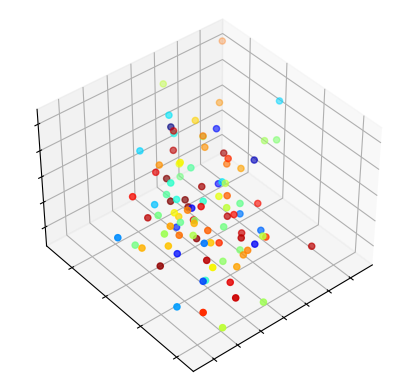
\includegraphics[width=0.2\textwidth]{img/avg/degrees_60000.png} &
        
\includegraphics[width=0.2\textwidth]{img/high/degrees_60000.png}  \\
        \hline
    \end{tabular}
    \caption{Distribution spatiale du degré}
    \label{fig:degrees}
\end{figure}

La distribution en valeur (figure \ref{fig:degree-hist}) est plus intéressante. À petite portée, peu de satellites sont très connectés, même à forte densité. En revanche, à grande portée, la distribution des degrés est inversée, les points isolés sont plus rare. Sur la densité et la portée maximale, on compte une quasi majorité de points de degré 25. On pourrait presque identifier les points isolés sur le graphe, qui gardent un faible degré malgré l'augmentation de la portée.

\begin{figure}[ht]
    \centering
    \begin{tabular}{|c|c|c|c|}
        \hline
        portée                                                               &
        faible densité                                                       &
        moyenne densité                                                      &
        haute densité                                                          \\
        \hline\hline
        $20 000$ km                                                          &
        
\includegraphics[width=0.2\textwidth]{img/low/degree-hist_20000.png} &
        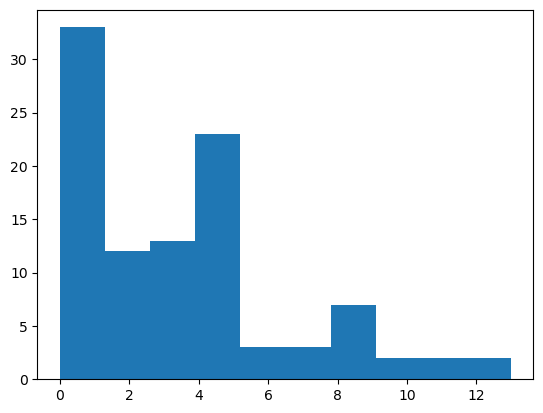
\includegraphics[width=0.2\textwidth]{img/avg/degree-hist_20000.png} &
        
\includegraphics[width=0.2\textwidth]{img/high/degree-hist_20000.png}  \\
        \hline
        $40 000$ km                                                          &
        
\includegraphics[width=0.2\textwidth]{img/low/degree-hist_40000.png} &
        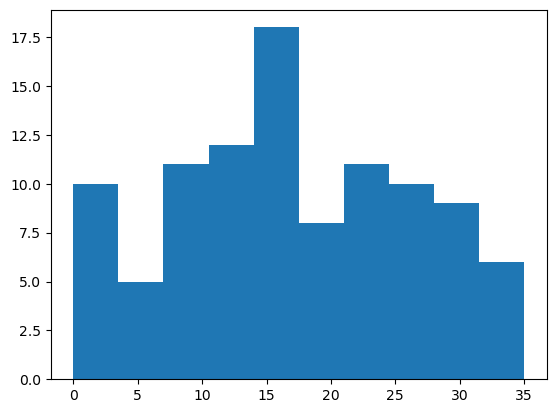
\includegraphics[width=0.2\textwidth]{img/avg/degree-hist_40000.png} &
        
\includegraphics[width=0.2\textwidth]{img/high/degree-hist_40000.png}  \\
        \hline
        $60 000$ km                                                          &
        
\includegraphics[width=0.2\textwidth]{img/low/degree-hist_60000.png} &
        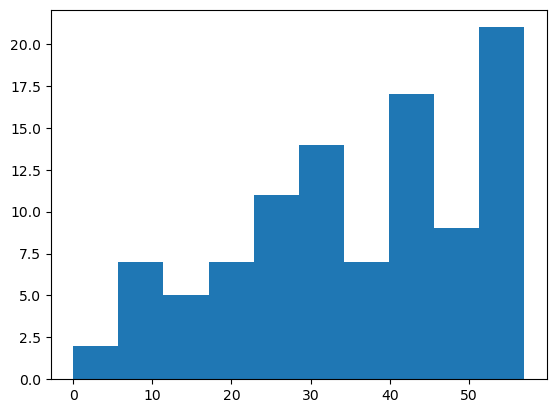
\includegraphics[width=0.2\textwidth]{img/avg/degree-hist_60000.png} &
        
\includegraphics[width=0.2\textwidth]{img/high/degree-hist_60000.png}  \\
        \hline
    \end{tabular}
    \caption{Histogrammes des degrés}
    \label{fig:degree-hist}
\end{figure}

\subsection{Degrés de clustering}

\begin{figure}[ht]
    \centering
    \begin{tabular}{|c|c|c|c|}
        \hline
        portée      & faible densité & moyenne densité & haute densité \\
        \hline\hline
        $20 000$ km & $0.23$         & $0.36$          & $0.40$        \\
        \hline
        $40 000$ km & $0.52$         & $0.64$          & $0.67$        \\
        \hline
        $60 000$ km & $0.67$         & $0.73$          & $0.73$        \\
        \hline
    \end{tabular}
    \caption{Moyennes des degrés de clustering en fonction de la portée et de la densité}
    \label{tab:clustering-degrees-mean}
\end{figure}

Le degré de clustering\footnote{\url{https://en.wikipedia.org/wiki/Clustering_coefficient}} a "souffert" du même doute que le degré.

La distribution spatiale du degré de clustering (figure \ref{fig:clustering-degrees}) est assez similaire à celle du degré. On remarque des valeurs bien plus grandes ou plus petites que d'autres. La cohésion locale des satellites est moins homogène que leur degré. Plus le nuage est intensément connecté, chaque satellite est sommet d'un triangle avec ses voisins. Un degré de clustering élevé est important dans notre cas car il signifie que la panne de l'un des trois satellites qui forment un triangle n'impacte en rien de flot de données transmissibles puisqu'il suffit de dérouter les données par un autre satellite du triangle.

\begin{figure}[ht]
    \centering
    \begin{tabular}{|c|c|c|c|}
        \hline
        portée                                                                      &
        faible densité                                                              &
        moyenne densité                                                             &
        haute densité                                                                 \\
        \hline\hline
        $20 000$ km                                                                 &
        
\includegraphics[width=0.2\textwidth]{img/low/clustering-degrees_20000.png} &
        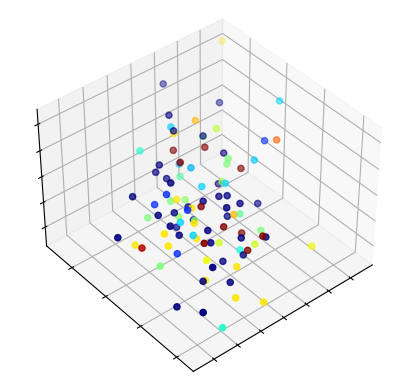
\includegraphics[width=0.2\textwidth]{img/avg/clustering-degrees_20000.png} &
        
\includegraphics[width=0.2\textwidth]{img/high/clustering-degrees_20000.png}  \\
        \hline
        $40 000$ km                                                                 &
        
\includegraphics[width=0.2\textwidth]{img/low/clustering-degrees_40000.png} &
        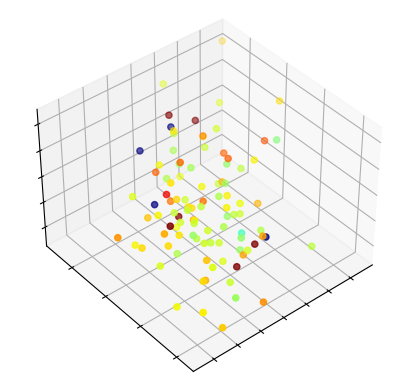
\includegraphics[width=0.2\textwidth]{img/avg/clustering-degrees_40000.png} &
        
\includegraphics[width=0.2\textwidth]{img/high/clustering-degrees_40000.png}  \\
        \hline
        $60 000$ km                                                                 &
        
\includegraphics[width=0.2\textwidth]{img/low/clustering-degrees_60000.png} &
        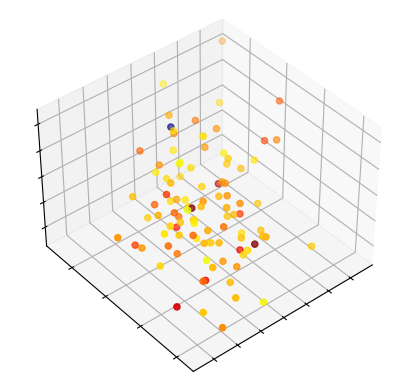
\includegraphics[width=0.2\textwidth]{img/avg/clustering-degrees_60000.png} &
        
\includegraphics[width=0.2\textwidth]{img/high/clustering-degrees_60000.png}  \\
        \hline
    \end{tabular}
    \caption{Distribution spatiale du degré de clustering}
    \label{fig:clustering-degrees}
\end{figure}

Cette fois encore, les histogrammes (figure \ref{fig:clustering-degree-hist}) renferment le plus d'information. Les degrés de clustering paraissent ne prendre qu'un nombre limité de valeurs concentrées. De manière cohérente, ces valeurs discrètes augmentent avec la portée.

\begin{figure}[ht]
    \centering
    \begin{tabular}{|c|c|c|c|}
        \hline
        portée                                                                          &
        faible densité                                                                  &
        moyenne densité                                                                 &
        haute densité                                                                     \\
        \hline\hline
        $20 000$ km                                                                     &
        
\includegraphics[width=0.2\textwidth]{img/low/clustering-degree-hist_20000.png} &
        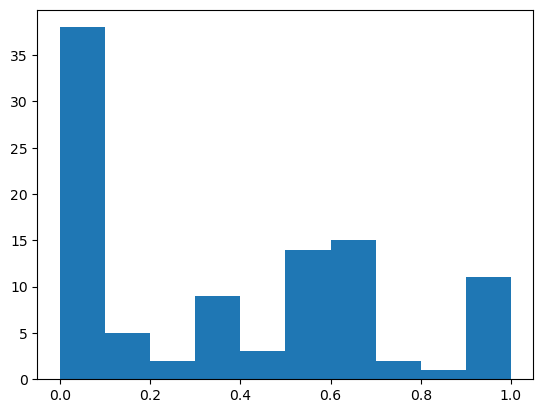
\includegraphics[width=0.2\textwidth]{img/avg/clustering-degree-hist_20000.png} &
        
\includegraphics[width=0.2\textwidth]{img/high/clustering-degree-hist_20000.png}  \\
        \hline
        $40 000$ km                                                                     &
        
\includegraphics[width=0.2\textwidth]{img/low/clustering-degree-hist_40000.png} &
        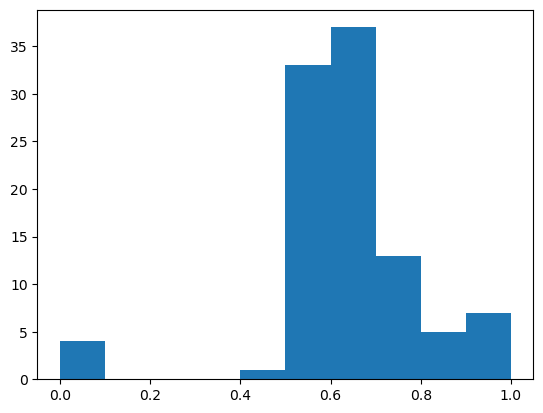
\includegraphics[width=0.2\textwidth]{img/avg/clustering-degree-hist_40000.png} &
        
\includegraphics[width=0.2\textwidth]{img/high/clustering-degree-hist_40000.png}  \\
        \hline
        $60 000$ km                                                                     &
        
\includegraphics[width=0.2\textwidth]{img/low/clustering-degree-hist_60000.png} &
        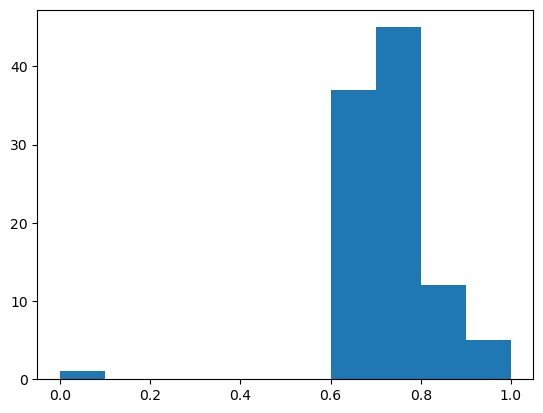
\includegraphics[width=0.2\textwidth]{img/avg/clustering-degree-hist_60000.png} &
        
\includegraphics[width=0.2\textwidth]{img/high/clustering-degree-hist_60000.png}  \\
        \hline
    \end{tabular}
    \caption{Histogrammes des degrés de clustering}
    \label{fig:clustering-degree-hist}
\end{figure}

\subsection{Cliques}

Pour ce qui est du nombre de cliques (figure \ref{tab:num-cliques}), on pense à une mauvaise lecture de lma documentation. Les nombres nous paraissent peu cohérents et le temps nous a manqué pour vérifier à la main sur de plus petits exemples.

\begin{figure}[ht]
    \centering
    \begin{tabular}{|c|c|c|c|}
        \hline
        portée      & faible densité & moyenne densité & haute densité \\
        \hline\hline
        $20 000$ km & $77$           & $83$            & $85$          \\
        \hline
        $40 000$ km & $147$          & $171$           & $139$         \\
        \hline
        $60 000$ km & $301$          & $258$           & $200$         \\
        \hline
    \end{tabular}
    \caption{Nombre de cliques en fonction de la portée et de la densité}
    \label{tab:num-cliques}
\end{figure}

\subsection{Composantes connexes}

Comme prévu, augmenter la portée augmente la conexité et diminue le nombre de composantes connexes (figure \ref{tab:num-connected-components}). L'idéal serait d'atteindre le graphe connexe, afinde garantir une possibilité de communiquer entre chaque paire de satellites.

\begin{figure}[ht]
    \centering
    \begin{tabular}{|c|c|c|c|}
        \hline
        portée      & faible densité & moyenne densité & haute densité \\
        \hline\hline
        $20 000$ km & $39$           & $22$            & $23$          \\
        \hline
        $40 000$ km & $8$            & $4$             & $4$           \\
        \hline
        $60 000$ km & $4$            & $2$             & $2$           \\
        \hline
    \end{tabular}
    \caption{Nombre de composantes connexes en fonction de la portée et de la densité}
    \label{tab:num-connected-components}
\end{figure}

La figure \ref{fig:connected-components} montre les composantes connexes des graphes. chaque couleur représente une arête d'une composante connexe différente. Avec une porté de $20\ 000$ km, les différences de densités sont évidentes. C'est lorsque la portée est augmentée que le graphe ne ressemble plus qu'à une gigantesque toile d'araignée monochrome puisqu'il n'existe plus de point isolé.

\begin{figure}[ht]
    \centering
    \begin{tabular}{|c|c|c|c|}
        \hline
        portée                                                                        &
        faible densité                                                                &
        moyenne densité                                                               &
        haute densité                                                                   \\
        \hline\hline
        $20 000$ km                                                                   &
        
\includegraphics[width=0.2\textwidth]{img/low/connected-components_20000.png} &
        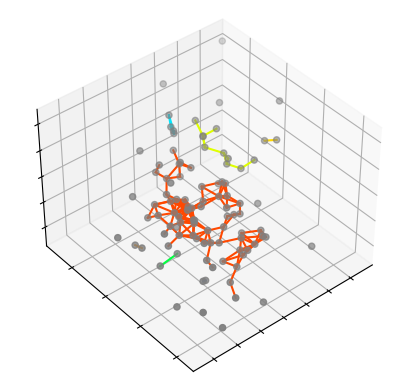
\includegraphics[width=0.2\textwidth]{img/avg/connected-components_20000.png} &
        
\includegraphics[width=0.2\textwidth]{img/high/connected-components_20000.png}  \\
        \hline
        $40 000$ km                                                                   &
        
\includegraphics[width=0.2\textwidth]{img/low/connected-components_40000.png} &
        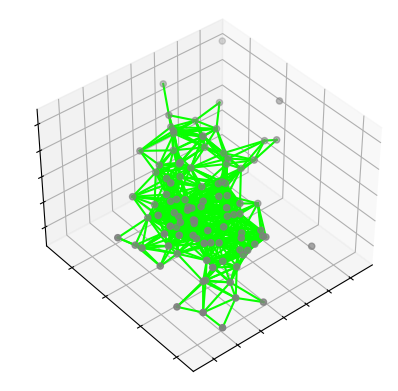
\includegraphics[width=0.2\textwidth]{img/avg/connected-components_40000.png} &
        
\includegraphics[width=0.2\textwidth]{img/high/connected-components_40000.png}  \\
        \hline
        $60 000$ km                                                                   &
        
\includegraphics[width=0.2\textwidth]{img/low/connected-components_60000.png} &
        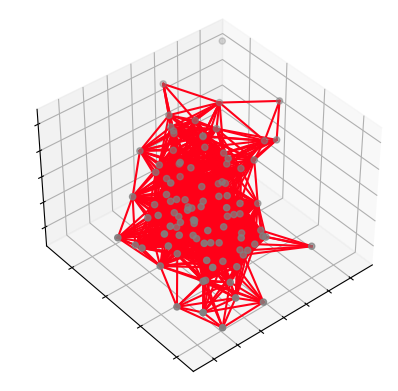
\includegraphics[width=0.2\textwidth]{img/avg/connected-components_60000.png} &
        
\includegraphics[width=0.2\textwidth]{img/high/connected-components_60000.png}  \\
        \hline
    \end{tabular}
    \caption{Composantes connexes (de couleurs différentes)}
    \label{fig:connected-components}
\end{figure}

\subsection{Plus courts chemins}

Ces figures sont les plus intéressantes, On remarque que l'augmen

\begin{figure}[ht]
    \centering
    \begin{tabular}{|c|c|c|c|}
        \hline
        portée                                                                        &
        faible densité                                                                &
        moyenne densité                                                               &
        haute densité                                                                   \\
        \hline\hline
        $20 000$ km                                                                   &
        
\includegraphics[width=0.2\textwidth]{img/low/shortest-path-hist_20000.png} &
        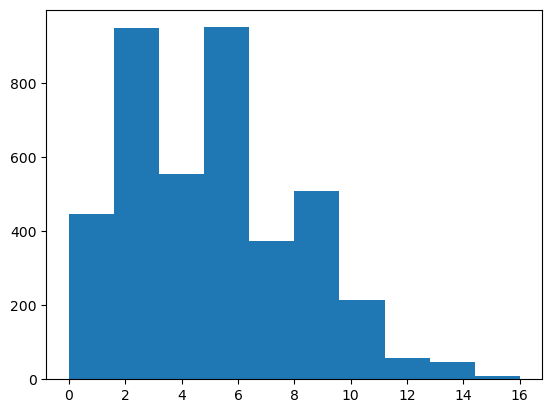
\includegraphics[width=0.2\textwidth]{img/avg/shortest-path-hist_20000.png} &
        
\includegraphics[width=0.2\textwidth]{img/high/shortest-path-hist_20000.png}  \\
        \hline
        $40 000$ km                                                                   &
        
\includegraphics[width=0.2\textwidth]{img/low/shortest-path-hist_40000.png} &
        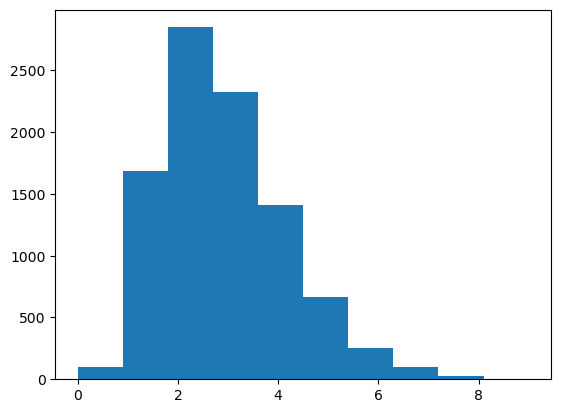
\includegraphics[width=0.2\textwidth]{img/avg/shortest-path-hist_40000.png} &
        
\includegraphics[width=0.2\textwidth]{img/high/shortest-path-hist_40000.png}  \\
        \hline
        $60 000$ km                                                                   &
        
\includegraphics[width=0.2\textwidth]{img/low/shortest-path-hist_60000.png} &
        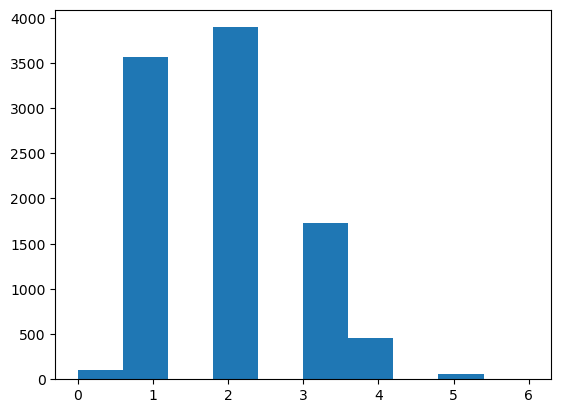
\includegraphics[width=0.2\textwidth]{img/avg/shortest-path-hist_60000.png} &
        
\includegraphics[width=0.2\textwidth]{img/high/shortest-path-hist_60000.png}  \\
        \hline
    \end{tabular}
    \caption{Distribution des longueurs des plus courts chemins}
    \label{fig:shortest-path-hist}
\end{figure}

\section{Partie 3 : Étude des graphes valués}

\end{document}